% SPDX-License-Identifier: Apache-2.0
\documentclass[11pt,letterpaper]{article}
\usepackage[T1]{fontenc}\usepackage[utf8]{inputenc}
\usepackage[margin=.88in,headheight=15pt]{geometry}
\usepackage{lmodern,microtype,amsmath,amssymb,booktabs,tabularx,longtable,array,graphicx,xcolor,fancyhdr,enumitem,xurl}
\definecolor{ink}{HTML}{142B42}\definecolor{accent}{HTML}{8C631D}
\usepackage[colorlinks=true,linkcolor=ink,citecolor=ink,urlcolor=ink]{hyperref}
\hypersetup{pdftitle={Profitable Work First. Compounding Capability When Worthwhile.},pdfauthor={AGI ALPHA computational research study},pdfsubject={Transformational Intelligence, Human-Market Value and Optional Alpha}}
\setlength{\parindent}{0pt}\setlength{\parskip}{.55em}\setlength{\emergencystretch}{2em}
\setlist{nosep,leftmargin=1.6em}\renewcommand{\arraystretch}{1.14}
\newcolumntype{Y}{>{\raggedright\arraybackslash}X}
\newcommand{\usd}[1]{\$#1}
\newcommand{\resultbox}[1]{\begin{center}\fcolorbox{ink}{ink!4}{\begin{minipage}{.94\linewidth}#1\end{minipage}}\end{center}}
\pagestyle{fancy}\fancyhf{}\fancyhead[L]{\small Profitable Work First}\fancyhead[R]{\small AGI ALPHA FLYWHEEL}\fancyfoot[C]{\thepage}
\begin{document}
\thispagestyle{plain}
\begin{center}
{\small\color{accent}\bfseries TRANSFORMATIONAL INTELLIGENCE $\infty$ \quad / \quad SUCCESSOR $\Omega$ HARNESS}\\[14pt]
{\Huge\bfseries\color{ink} AGI ALPHA FLYWHEEL}\\[9pt]
{\LARGE Profitable Work First. Compounding Capability When Worthwhile.}\\[10pt]
{\large Transformational Intelligence, Human-Market Value and Optional Alpha}\\[9pt]
{\small\bfseries FIND YOUR ALPHA. BUILD YOUR SUCCESSOR $\Omega$.}\\[5pt]
{\small ACTIVATE. EVOLVE. SCALE.}\\[12pt]
Computational research edition\quad$\cdot$\quad 27 October 2026\\[5pt]
\textbf{Enterprise outcomes are simulated. Local mechanism experiments were executed.}
\end{center}
\begin{abstract}
Expert current frontier AI may already provide a commercially valuable operating core. We study automated delivery of complete configurable optimization engines for bounded digital operations, using equivalent human-team service as the commercial reference. Competent frontier models, ordinary tools and existing local artifacts form \emph{Beta}. Profitability requires useful accepted work, customer choice, actual modeled collections and complete costs, including failures, automated validation, business overhead, discovery and reserves. Additional retained \emph{Alpha}, network sharing and further investment are optional enhancements, tested separately under matched conditions. Source-job learning is charged once in A; only extra retention and reuse enters B, and separate research enters C. Published tariffs and service rates anchor monetary units; effort, task reliability and buyer response remain explicit assumptions. Across 500 independent worlds per condition, central Beta-only delivery produced mean complete pre-tax profit of \usd{522,787}, 54.7 truly accepted projects, and \usd{489,833} available at month 24 after protecting reserves, known obligations and the original seed. Mean gross charge in the useful, collected cohort was \usd{10,870} against a scope-matched human reference of \usd{26,952}; pooled complete cost was \usd{1,020} per truly accepted outcome. Favorable Beta profit was \usd{3,421,787}; the conservative mean was \usd{-3,976}. Residual material false-pass rates were 6.3\% centrally and 1.3\% favorably. No primary world purchased additional retention or separate capability construction. Paid candidate scanning reduced network-policy profit slightly; that result does not negate profitable Beta operation. A separately frozen exploratory belief diagnostic enabled useful reuse but remained less profitable than Beta after complete costs. These are conditional modeled economics, not observed sales, operational certification or demonstrated recursive improvement.

\end{abstract}
\textbf{Keywords:} transformational intelligence; frontier AI; validated Alpha; capability networks; posted-price games; finite cash; endogenous investment.

\section{The business mechanism and the answer it supports}
\resultbox{\textbf{Profitable work is the primary result.} Central Beta-only operation earned mean complete pre-tax profit of \usd{522,787} and retained \usd{489,833} at month 24 above the original seed, reserves and known obligations. Favorable mean profit was \usd{3,421,787}. The conservative condition lost \usd{3,976} on average. Optional Alpha is a separate economic question: the primary network policy changed central profit by \usd{-79}. A profitable Beta-only enterprise is a valid positive commercial result; profitable delivery is not evidence of capability compounding.}


The opportunity is to sell a useful decision instrument. A buyer needs to allocate changing tasks to limited resources while respecting eligibility and capacity. A configurable engine, its explicit model and independent checks can continue to support those decisions. During delivery, an agent may learn a representation or evidence protocol that helps another project. Revenue exists only when the buyer purchases and collection occurs. The resulting artifact is not automatically Alpha: extracting, generalizing, testing and sharing it must add net value on fresh work. A job can be profitable without leaving a useful skill, and a useful artifact can emerge before the originating invoice clears.

The commercial reference is competent multidisciplinary human delivery over a comparable scope. It asks whether \textbf{Beta economics} are attractive. The causal reference is the same network with competent Beta, including ordinary source-job artifacts, but without newly admitted portable skills. It asks whether \textbf{retained Alpha} adds value. A third comparison asks whether sharing improves on private retention at the same aggregate resources. A profitable job's construction cost remains in the enterprise ledger; prospective admission does not charge that cost again. Sharing can benefit one recipient and be redundant for another. No comparison requires superiority over an unrelated AI system.

The complete package contains the economic network simulator, all confirmation histories, frozen decision rules, a tested graph lifecycle and access-policy implementation, a source-linked calibration register, Beta/Alpha and sharing ablations, a bounded local mathematical witness, an English/French offline demonstration and this paper's source. No customer purchases, frontier API job executions, real ENS identity checks or deployed self-improvement are reported.

\section{Commercial results first; optional enhancements separately}
The behavioral protocol, costs and stress design were frozen before confirmation on 26 October 2026 at 23:55 UTC (full timestamp in the freeze manifest). There are 500 independent world IDs per primary condition and four matched policies: 1,500 condition--world evaluations and 6,000 complete policy histories. Conditions reuse keyed random streams; the condition ensembles are not mutually independent. Confirmation seed 951251 is distinct from development seed 951043. Each history includes paid discovery/setup, 24 operating months and three settlement-runoff months. Every world is preserved. The enterprise campaign is the experimental unit; descendant jobs are not additional independent inventions.

Configuration SHA-256: \nolinkurl{051f7f528c1bce29f1e83b22ebb8da9b4fc3efd1dc62f6f7936912475636f98a}. The commercial-core-first presentation requested on 27 October changes no frozen parameter, policy, hypothesis, seed or outcome. Monetary tariffs retain their 26 October evidence cutoff. Future Beta epochs are assumptions, not forecasts of named releases. Reported distributions describe these specified simulated populations, not empirical probabilities of commercial success.

\subsection{Beta-only useful delivery and complete profit}
Competent Beta includes the current frontier workflow, ordinary tools, existing equivalents and useful source-agent local artifacts. It requires no newly admitted graph skill and no optional capability campaign. The following commercial results stand independently of the optional Alpha findings.
\begin{table}[htbp]\centering\small\begin{tabular}{lrrrrr}
\toprule
Condition & Useful jobs & Human ref.* & Charge* & Cost/useful & Net profit\\\midrule
Conservative & 4.2 & \usd{15,228} & \usd{4,639} & \usd{5,405} & \usd{-3,976}\\
Central & 54.7 & \usd{26,952} & \usd{10,870} & \usd{1,020} & \usd{522,787}\\
Favorable & 150.2 & \usd{43,875} & \usd{24,034} & \usd{1,059} & \usd{3,421,787}\\
\bottomrule\end{tabular}\caption{Beta-only commercial core. Project counts and complete profit are enterprise means. *Human reference and gross charge use the same truly useful, collected cohort, including richer scopes. Complete cost pools all paid and failed work, overhead, setup and discovery over all truly accepted outcomes, including valid outcomes whose payment was not authorized. The columns are not an algebraic per-job profit calculation. USD; simulated.}\end{table}
\begin{table}[htbp]\centering\small\begin{tabular}{lrrrrr}
\toprule
Condition & Collections & Refunds & All costs & Profit 5th & Profit 95th\\\midrule
Conservative & \usd{23,222} & \usd{4,378} & \usd{22,820} & \usd{-19,238} & \usd{15,082}\\
Central & \usd{609,327} & \usd{30,748} & \usd{55,792} & \usd{225,770} & \usd{951,875}\\
Favorable & \usd{3,616,321} & \usd{35,451} & \usd{159,083} & \usd{2,109,877} & \usd{5,157,358}\\
\bottomrule\end{tabular}\caption{Mean settled gross receipts, paid refunds and complete costs; profit distribution across all worlds. Fees are already in costs. Unpaid refund liabilities also reduce profit. Seed capital is not revenue.}\end{table}

\textbf{Conservative.} Beta delivered 4.2 truly useful projects (0.18 per operating month), of which 3.8 were useful and collected. The gross charge in that paid cohort averaged \usd{4,639}; its matched human reference averaged \usd{15,228}. Their arithmetic reference-price difference was \usd{10,589}, or a mean 69.5\% discount across those projects. This is not observed buyer savings or proof that every buyer would otherwise purchase the human service. The mean monthly posted base-scope price was \usd{4,237} (32.6\% of the base reference), distinct from the sold scope mix. The modeled purchase share was 25.9\% across 24.4 qualified opportunities. Profit was positive in 31.0\% of simulated worlds; cash-shortfall shutdown occurred in 2.4\%. These are scenario frequencies, not calibrated real-world success probabilities.

\textbf{Central.} Beta delivered 54.7 truly useful projects (2.28 per operating month), of which 52.5 were useful and collected. The gross charge in that paid cohort averaged \usd{10,870}; its matched human reference averaged \usd{26,952}. Their arithmetic reference-price difference was \usd{16,083}, or a mean 59.7\% discount across those projects. This is not observed buyer savings or proof that every buyer would otherwise purchase the human service. The mean monthly posted base-scope price was \usd{9,353} (40.9\% of the base reference), distinct from the sold scope mix. The modeled purchase share was 58.6\% across 109.2 qualified opportunities. Profit was positive in 100.0\% of simulated worlds; cash-shortfall shutdown occurred in 0.0\%. These are scenario frequencies, not calibrated real-world success probabilities.

\textbf{Favorable.} Beta delivered 150.2 truly useful projects (6.26 per operating month), of which 148.6 were useful and collected. The gross charge in that paid cohort averaged \usd{24,034}; its matched human reference averaged \usd{43,875}. Their arithmetic reference-price difference was \usd{19,841}, or a mean 45.2\% discount across those projects. This is not observed buyer savings or proof that every buyer would otherwise purchase the human service. The mean monthly posted base-scope price was \usd{20,337} (54.7\% of the base reference), distinct from the sold scope mix. The modeled purchase share was 66.7\% across 245.7 qualified opportunities. Profit was positive in 100.0\% of simulated worlds; cash-shortfall shutdown occurred in 0.0\%. These are scenario frequencies, not calibrated real-world success probabilities.

\textbf{Quality is a separate condition.} Material errors among approved Beta deliveries were 23.5\%, 6.3\% and 1.3\% in conservative, central and favorable conditions. Removing all otherwise undetected paid false-pass receipts as a terminal valuation stress leaves central profit of \usd{515,390} and favorable profit of \usd{3,411,472}. This supports the modeled useful-work margin without treating erroneous receipts as indispensable. It does not create a new refund-timing trajectory, establish a full liability ceiling, or prove that buyers accept the residual error rate. A required error budget tighter than a scenario's residual rate would require a stronger validator or narrower offering.

\subsection{Available surplus, seed and throughput}
\begin{table}[htbp]\centering\scriptsize\begin{tabular}{lrrrrr}
\toprule
Condition & Cash, m24 & Reserve, m24 & Receivable, m24 & Excess*, m24 & Excess*, m27\\\midrule
Conservative & \usd{14,946} & \usd{2,166} & \usd{1,726} & \usd{1,766} & \usd{2,412}\\
Central & \usd{519,077} & \usd{9,243} & \usd{27,260} & \usd{489,833} & \usd{516,107}\\
Favorable & \usd{3,260,307} & \usd{38,830} & \usd{190,726} & \usd{3,201,477} & \usd{3,386,459}\\
\bottomrule\end{tabular}\caption{Beta cash stocks, USD means. *Nonnegative cash available after protecting known obligations, the declared reserve and the entire original USD20,000 seed. Receivables cannot fund current spending. Known refunds/recovery are not subtracted twice when already inside reserve. The settled endpoint retains the operating reserve policy; it is not liquidation value. Nonnegative world-level stocks are averaged, so a positive mean excess does not negate conservative losses.}\end{table}
Central month-24 uncommitted cash was \usd{509,833}, including possible seed, while \usd{489,833} remained after preserving the entire seed. Its 5th--95th percentile range above seed was \usd{209,585} to \usd{883,502}. The conservative median excess above seed was zero even though many enterprises retained some original capital. These stocks differ from accrual-like complete profit and are never summed across months.
The primary runs show no capacity-deferred orders. Their achieved throughput therefore demonstrates conditional operation at the tested demand, not a measured saturation point or an Alpha-driven capacity expansion. The resource screens and scale stresses locate conditional bottlenecks; actual provider quotas, latency and validator capacity require later measurement. Increased volume by itself is not self-acceleration.
\begin{figure}[htbp]\centering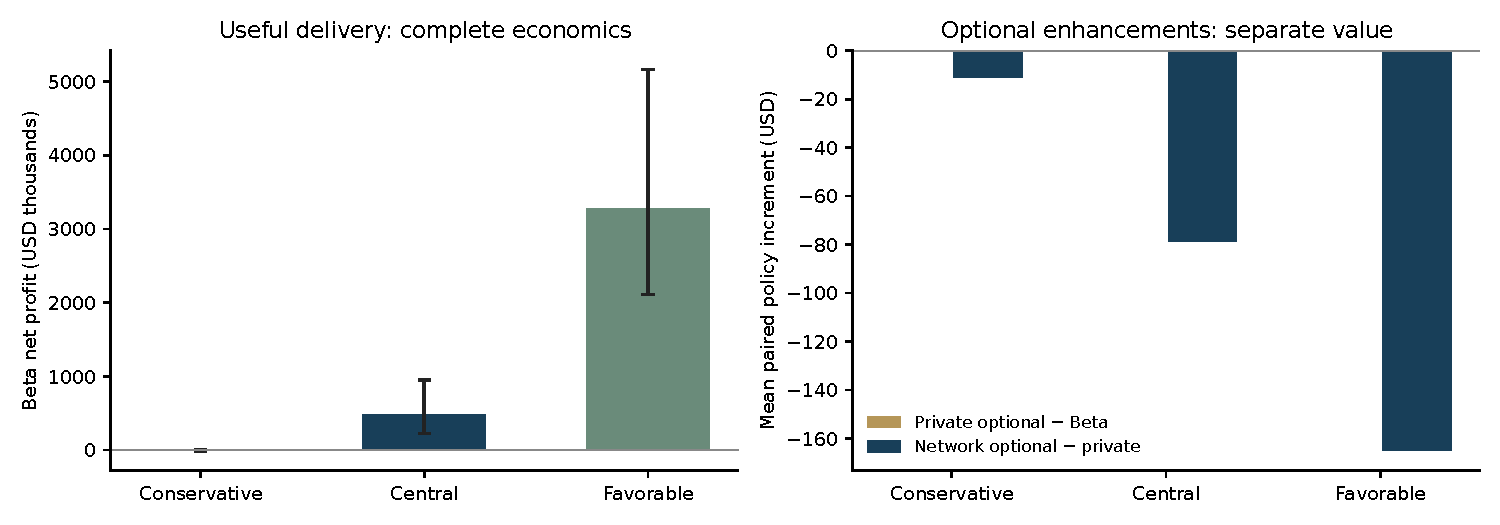
\includegraphics[width=\linewidth]{generated/results_overview.pdf}\caption{Commercial core first. Left: Beta complete-profit medians and 5th--95th percentile ranges. Right: paired mean policy increments from optional private capability decisions and network availability. The scales differ deliberately: large service economics and small enhancement effects are distinct questions.}\end{figure}
\subsection{Optional retained Alpha, sharing and investment}
\begin{table}[htbp]\centering\small\begin{tabular}{lrrrrr}
\toprule
Condition & Network $-$ Beta & Network $-$ private & Retain & Admit & Feedback\\\midrule
Conservative & \usd{-11} & \usd{-11} & 0.0\% & 0.00 & 0.0\%\\
Central & \usd{-79} & \usd{-79} & 0.0\% & 0.00 & 0.0\%\\
Favorable & \usd{-165} & \usd{-165} & 0.0\% & 0.00 & 0.0\%\\
\bottomrule\end{tabular}\caption{Optional-policy mean increments and all-world frequencies, kept separate from Beta commercial success. Retain is an additional B-package purchase. Feedback requires an operating-funded package linking useful collected source work to useful fresh recipient work, positive total and quality-adjusted paired value, and no separate C construction campaign. It is descriptive, not a mandatory investment count.}\end{table}
No primary world purchased portable retention or optional separate capability construction. Ordinary source-agent artifacts remain available under Beta; paid candidate scans and nominated candidates do not establish additional Alpha. The tested policy declined the incremental expenditures. Its small negative network effects reflect the cost and incidental resource consequences of searching, not destruction of the profitable commercial core. This is evidence of the tested policy choosing restraint, not proof that every possible retained capability is worthless or that global optimality has been established.

Conservative: network availability changed mean profit by \usd{-11} (Monte Carlo standard error \usd{0.41}; 5th--95th percentile \usd{-27} to \usd{0}). Private optional decisions changed profit by \usd{0}. Paid scans averaged 1.9, nominated candidates 0.3, and upfront B purchases \usd{0}. There were 0.00 useful capability--project reuse pairs; separate capsules can create multiple pairs for one project. The paired policy effect on distinct useful projects was 0.00. Endogenous network pricing changed mean profit by \usd{8,404} relative to the fixed 65\% diagnostic; this comparison includes any induced resource decisions.

Central: network availability changed mean profit by \usd{-79} (Monte Carlo standard error \usd{1.60}; 5th--95th percentile \usd{-148} to \usd{-31}). Private optional decisions changed profit by \usd{0}. Paid scans averaged 20.4, nominated candidates 2.0, and upfront B purchases \usd{0}. There were 0.00 useful capability--project reuse pairs; separate capsules can create multiple pairs for one project. The paired policy effect on distinct useful projects was 0.00. Endogenous network pricing changed mean profit by \usd{161,153} relative to the fixed 65\% diagnostic; this comparison includes any induced resource decisions.

Favorable: network availability changed mean profit by \usd{-165} (Monte Carlo standard error \usd{2.13}; 5th--95th percentile \usd{-250} to \usd{-94}). Private optional decisions changed profit by \usd{0}. Paid scans averaged 53.3, nominated candidates 3.0, and upfront B purchases \usd{0}. There were 0.00 useful capability--project reuse pairs; separate capsules can create multiple pairs for one project. The paired policy effect on distinct useful projects was 0.00. Endogenous network pricing changed mean profit by \usd{176,018} relative to the fixed 65\% diagnostic; this comparison includes any induced resource decisions.
\begin{table}[htbp]\centering\small\begin{tabular}{lrrrrr}
\toprule
Condition & Beta A & Beta B & Beta C* & Network B & Later C\\\midrule
Conservative & \usd{17,569} & \usd{0} & \usd{5,251} & \usd{11} & \usd{0}\\
Central & \usd{50,541} & \usd{0} & \usd{5,251} & \usd{79} & \usd{0}\\
Favorable & \usd{153,833} & \usd{0} & \usd{5,251} & \usd{165} & \usd{0}\\
\bottomrule\end{tabular}\caption{Disjoint complete-cost records, USD means. A includes delivery, within-job learning, qualification, fees and allocated overhead. B includes extra scans, failed candidates, retention and reuse. *C includes initial bounded venture discovery; later optional C campaigns are identified separately. Refunds reverse revenue, and no source-job construction is charged again to B.}\end{table}
The primary confirmation does not supply a population of funded admissions from which to estimate admission precision or realized skill repayment. Directed funded and recovery fixtures verify software/accounting branches only; their forced capital action is not economic-selection evidence. Any actual funded sensitivity path is separately labeled and retains its all-world frequency. Profitable delivery, useful retained Alpha, productive reinvestment and self-acceleration remain different claims.

\subsection{Conditional break-even screens}\begin{table}[htbp]\centering\small\begin{tabular}{lrrrr}
\toprule
Condition & Useful / month & Required purchase & Validation ceiling* & Capacity upper*\\\midrule
Conservative & 0.229 & 38.0\% & \usd{3,068} & 13.4\\
Central & 0.086 & 2.8\% & \usd{9,196} & 22.0\\
Favorable & 0.039 & 0.6\% & \usd{22,016} & 29.1\\
\bottomrule\end{tabular}\caption{Analytic screens at the confirmation mean posted price. *Validation ceiling is per useful outcome at one useful project/month; capacity is purchased project attempts/month before bursts, queues, retention and maintenance. Complete setup, settlement-runoff overhead and qualification are included; all false passes are refunded in this screen. These are conditional thresholds, not demand evidence or service guarantees.}\end{table}
The primary retention options cost \usd{290.05} for R, \usd{307.95} for V, \usd{569.72} for bundle. Their optimistic reconstruction-only reuse requirements are 5.2 for R, 8.3 for V, 6.2 for bundle. The source job is not charged again. Actual repayment requires enough compatible first encounters with recipients after overlap, transfer, access, upkeep, erosion and the capacity consumed by retention.

For an additional retention bill $K$, maximum affordable expenditure at a decision is cleared cash minus protected liabilities, reserves and headroom. The full ledger determines this ceiling before spending. For constant compatible reuse $u$ and per-use incremental value $b_t$, the prospective screen is $\sum_{t=1}^{H}\delta^t(ub_t-m_t)>K$, where $m_t$ includes remaining maintenance and revalidation. Advancing Beta changes $b_t$; a shorter useful lifetime or lower adoption can make waiting optimal even after a profitable source job.

\subsection{Prespecified sensitivity and ablation results}
The 19 frozen conditions each use 200 independent world IDs and four matched policies. The common stress seed is 951352, separate from the primary confirmation seed. Conditions reuse keyed random streams: there are 3,800 case--world evaluations, not that many mutually independent draws. Every condition and all scalar world outcomes are preserved. Compound changes are explicitly exploratory scenarios, declared before confirmation; they are not isolated causal estimates or calibrated demand forecasts.
\begin{table}[htbp]\centering\scriptsize\begin{tabular}{p{.37\linewidth}rrrr}
\toprule
Condition & Beta profit & Network $-$ Beta & Retention & Admission\\\midrule
Human reference USD 4,900 (C) & \usd{80,729} & \usd{-75} & 0.0\% & 0.0\%\\
One opportunity per month & \usd{311,873} & \usd{-17} & 0.0\% & 0.0\%\\
No job-born candidates & \usd{3,366,012} & \usd{0} & 0.0\% & 0.0\%\\
No separate C research & \usd{3,366,012} & \usd{-160} & 0.0\% & 0.0\%\\
Zero incremental Alpha effects & \usd{3,366,012} & \usd{0} & 0.0\% & 0.0\%\\
Nominal cost-only effects (qualified) & \usd{3,366,012} & \usd{-160} & 0.0\% & 0.0\%\\
All recipients already equivalent & \usd{3,374,109} & \usd{-160} & 0.0\% & 0.0\%\\
Ordinary cross-agent reuse is free & \usd{3,371,504} & \usd{-160} & 0.0\% & 0.0\%\\
Static Beta & \usd{3,365,763} & \usd{-160} & 0.0\% & 0.0\%\\
Faster Beta erosion & \usd{3,368,094} & \usd{-160} & 0.0\% & 0.0\%\\
48 recipients; same compute & \usd{3,401,705} & \usd{-176} & 4.5\% & 1.0\%\\
Specialist routing; same compute & \usd{3,366,179} & \usd{-160} & 0.0\% & 0.0\%\\
Concentrated supported schema & \usd{3,379,446} & \usd{25} & 0.0\% & 0.0\%\\
Double validation activities & \usd{3,351,553} & \usd{-4} & 0.0\% & 0.0\%\\
Double retention activities & \usd{3,366,012} & \usd{-160} & 0.0\% & 0.0\%\\
Stronger correlated errors (C) & \usd{340,246} & \usd{-71} & 0.0\% & 0.0\%\\
80\% authorization, two-month lag (C)* & \usd{413,350} & \usd{-78} & 0.0\% & 0.0\%\\
Looser capacity; quality effects retained & \usd{3,365,422} & \usd{-160} & 0.0\% & 0.0\%\\
Joint static-Beta / larger-pool case* & \usd{10,723,148} & \usd{-1,380} & 93.5\% & 44.0\%\\
\bottomrule\end{tabular}\caption{All prespecified stresses, USD means and all-world frequencies. (C) changes the central condition; other rows change the favorable condition. *Compound scenario. Retention is any additional B purchase; admission is any paid-job capsule admitted within the simulation. No frozen sensitivity produces actual capsule reuse or operating-funded useful feedback. These capability results are qualified by the recipient decision bottleneck described below.}\end{table}

\textbf{Redundancy and attribution.} Removing the modeled Alpha effects changes network profit relative to Beta by \usd{0}; making every recipient equivalent yields \usd{-160}. When ordinary cross-agent reuse is itself free and equivalent, the increment is \usd{-160}. These controls test whether the formal sharing layer adds anything beyond capabilities already available. The nominal cost-only case produces \usd{-160}, but a recipient-valuation defect prevents interpreting it as a clean quality-free ablation. Reliability-linked dollar value must not be inferred solely from avoided token costs.

\textbf{The moving frontier and the recipient pool.} Static Beta produces a mean increment of \usd{-160}, versus \usd{-160} under faster erosion. Forty-eight heterogeneous recipients at unchanged aggregate compute produce \usd{-176}; this isolates recipient-pool structure from simply buying more compute. The joint scenario produces \usd{-1,380}, with useful operating-funded feedback in 0.0\% of worlds. It jointly holds Beta static, expands the recipient pool, increases paid-contract arrivals and pays for fourfold reserved capacity/control resources. Its result cannot be attributed to any one of those changes.

\textbf{Commercial failure conditions.} At the USD 4,900 human reference, mean Beta profit is \usd{80,729}; with one monthly opportunity it is \usd{311,873}. Stronger correlated errors leave 20.1\% material errors among approved deliveries and mean Beta profit of \usd{340,246}. Positive accounting profit alone does not establish an acceptable error rate, buyer trust or product fitness.

The frozen identifier \texttt{loose\_capacity\_cost\_only} changes reserved capacity but retains quality effects; it is therefore labeled accordingly in the table. The distinct \texttt{cost\_only\_alpha} case removes the quality increment. No frozen parameters were changed to repair that naming ambiguity. The primary candidate-scan frequency and one-campaign forecast are bounded heuristics; a policy that stops unproductive searching may do better. No global optimum is claimed.

\textbf{What the frozen Alpha result cannot establish.} The 48-recipient, same-compute case purchases retention in 4.5\% of worlds and admits it in 1.0\%; the compound case purchases in 93.5\% and admits in 44.0\%. Neither produces a capsule use. A post-confirmation independent review found that recipient beliefs and admission forecasts are not harmonized. The candidate posterior mean $(2+s)/(4+n)$ has a ceiling of $26/28=0.92857$ after 24 perfect cases, or $18/20=0.90$ after a 16-case reassessment. It is compared with a known favorable Beta component correctness of at least $0.97$. Even at the lowest permitted price and greatest reconstruction saving, the resulting favorable per-use valuation is negative before acquisition costs. Zero uptake is therefore structurally imposed by this conservative trust rule, rather than evidence that every underlying capability lacks incremental value. Admission and capital forecasts can still expect deployment, creating a controller mismatch.

The frozen cost-only ablation also omits the quality-effect multiplier from recipient valuation, so it can charge a perceived quality penalty although the deployed capability has no modeled quality effect. All frozen outcomes and hashes are preserved; this limitation does not alter Beta-only delivery, cash or profit. The positive USD24.78 increment in the concentrated-schema case has no retention purchase or reuse and is an incidental whole-policy resource/cash effect, not evidence of Alpha.

A deterministic replay of the lowest-ID admitted compound world matches all 95 saved scalar and paired fields. It spends USD232.04 on an admitted package, uses it zero times, and loses USD843.61 relative to Beta. This is an admitted-but-unused mechanism diagnostic, not a new trial. The separate directed QA transfer fixture exercises a useful fresh-recipient branch but loses USD450.05 over the whole paired trajectory; its forced action is never commercial-selection evidence. One fresh-sample posterior-coherence diagnostic is declared separately; it changes beliefs, not actual model capability, and cannot replace the frozen primary or stress findings.

\IfFileExists{generated/exploratory_coherence.tex}{\subsection{One exploratory recipient-belief diagnostic}
After the frozen zero-use result was diagnosed, one new protocol was frozen before a single fresh run: 100 matched world IDs, seed 951557, and three arms (300 complete histories). It uses the previously declared compound condition, with static Beta, 48 recipients, greater contract recurrence and paid additional capacity. This is a post-confirmation exploratory belief sensitivity, not replacement confirmation or evidence of a real market.

The treatment preserves the actual task, capability, failure, cost, cash, demand and resource generators. It retains four prior-equivalent cases but centers the prior on declared construction assumptions: $q_0=\pi q_{\rm good}+(1-\pi)0.65$ and $\hat q=(4q_0+s)/(4+n)$. For a paid-job capsule, $\pi$ is declared reconstruction correctness times retention-generalization success; for separate research it is declared build success. No latent source truth or future outcome is available to the controller. This prior is an unmeasured decision assumption, not a capability bonus. The extension also honors the quality-effect multiplier in reuse valuation; it equals one here and cannot cause this treatment difference.
\begin{table}[htbp]\centering\small\begin{tabular}{lrrrr}
\toprule
Arm & Profit $-$ Beta & Admission & Useful reuse & Useful pairs\\\midrule
Frozen Beta & \usd{0.00} & 0.0\% & 0.0\% & 0.00\\
Frozen network & \usd{-1,300.19} & 38.0\% & 0.0\% & 0.00\\
Declared-prior network & \usd{-1,172.65} & 38.0\% & 36.0\% & 1.53\\
\bottomrule\end{tabular}\caption{Fresh exploratory diagnostic. Frequencies use all 100 worlds. Useful pairs are capsule--project pairs, not necessarily distinct projects. Beta mean complete profit is \usd{11,073,182} in this deliberately strong compound condition. All inputs, full ledgers and negative outcomes are retained.}\end{table}
The declared-prior policy produces useful reuse in 36.0\% of worlds, with 1.71 attempted and 1.53 useful capsule--project uses per world. Admission occurs in 38.0\% of worlds. Relative to the frozen network it improves mean profit by \usd{127.54} (median \usd{0}; 5th--95th percentile \usd{0} to \usd{543.53}; minimum \usd{-152.43}). The revised belief opens a previously blocked reuse path; it does not guarantee a worthwhile retention policy.

\textbf{Beta remains the best tested policy.} The declared-prior network loses \usd{1,172.65} on average relative to Beta (Monte Carlo standard error \usd{42.53}; median \usd{-1,180.54}; 5th--95th percentile \usd{-1,894.47} to \usd{-589.85}). It underperforms Beta in every one of the 100 worlds. Quality-adjusted differences are identical. The paired change in distinct useful accepted projects is zero. Mean extra B spending is \usd{1,254.70}, including rejected candidates and upkeep. Useful transfer is therefore demonstrated within this simulation, but total retention-policy repayment and operating-funded profitable feedback remain unsupported. Both network arms also undertake one optional C campaign in one world; its cost remains in total policy profit (mean USD47.68 across all worlds). These contrasts therefore measure whole-policy effects, not the isolated repayment of each capsule.

This single diagnostic separates a software decision bottleneck from economic success: correcting the belief mismatch can enable useful reuse without making the complete enhancement worthwhile. No further policy or parameter tuning followed. The primary Beta result is unchanged, and no volume, graph size, reuse count or profitable source job is relabeled as recursive improvement. The separately frozen files, four directed extension tests and independent 300-history cash/provenance audit accompany the result.
}{}


\section{A fresh scientific question grounded in transformational intelligence}
The supplied manuscript, \emph{Transformational Intelligence: Learning to Change the Game}, separates authorized purpose, inherited formulation and evaluation instrument~\cite{TI}. The Gym, Specialist ASI and Successor $\Omega$ foundation distinguishes a candidate institution from admitted authority and separates the working system from protected evaluation~\cite{GymOmega,EnterpriseOmega}. We use these as research foundations, not evidence of deployed autonomous venture creation. Our user-defined Beta means competent frontier capability; it is not the Gym manuscript's separate factor-sensitivity definition of Mission Beta. The TI manuscript's finite causal example is researcher specified and matched by an unrestricted planner; it does not calibrate commercial performance. Proposed formal thresholds or governance arrangements in foundation drafts do not override this study's explicit economic and authority boundaries.

Our charter is to create useful, correctly scoped executable decision systems and allocate resources sustainably. The formulation is allowed to change: from repeatedly rebuilding a single-purpose program to constructing a parametric representation with evidence produced alongside its outputs. The commercial objective does not change when this happens. Original constraints, customer usefulness, full cost, cash and permissions remain the reference.

Five hypotheses organize the study. H-Beta concerns profitable complete delivery against human services. H-Alpha concerns a positive increment from optional retained capabilities after complete costs. H-Share concerns extra value from network availability over private retention at equal resources. H-Erosion concerns loss or survival of that increment as Beta changes. H-Authority concerns lifecycle and reuse boundaries within the tested research software. Pricing and investment condition on observable evidence and cash. No hypothesis requires a prescribed number of investments.

Let $B_v$ denote competent Beta at model/tool epoch $v$, and $A_i$ a recipient's existing capabilities. For candidate $S$ and declared mission scope $z$, define
\begin{equation}
\Delta_{i,z}(S\mid v,A_i)=\mathbb{E}[U_z(B_v,A_i\cup S)-U_z(B_v,A_i)]-C^{\mathrm{acquire,use,risk}}_{i,z}.
\end{equation}
The authorized mission utility $U_z$ is unchanged. Prospective Alpha subtracts remaining incremental extraction, generalization, validation, integration, distribution, upkeep and capacity opportunity costs over a declared reuse horizon. The originating job's already-accounted-for construction is not subtracted again. Full enterprise economics still include every delivery and learning cost once. Alpha is conditional on scope, alternatives and evidence, not an intrinsic property of a file. Complementary bundles are valued jointly with their dependencies intact.

An admission is an evidence claim, not a guarantee. The record identifies the source job, already charged activities, competent comparison, fresh tests, uncertainty, compatible reuse and remaining costs. Simulated assessments can be wrong, so realized paired value is separate. Historical optional research remains in its own repayment account; a prospective admission or continuation decision compares future benefits with avoidable future costs. Acceptance, admission, capital allocation and operational authority are distinct decisions.

The transformational journey is made operational: \textbf{Identify} a buyer's binding restriction; \textbf{Out-Learn} through paid information and experiments; \textbf{Out-Think} through grounded representations and hypotheses; \textbf{Out-Design} an executable product; \textbf{Out-Strategise} on price, cash and retention; \textbf{Out-Execute} with automated checking and correction; and \textbf{Out-Evolve} through fresh-work tests, sharing and requalification. These are modeled work stages, not seven empirically established superhuman abilities.

We evaluate useful outcomes, profitability, liquidity, quality, retained capabilities and new supported offerings separately. A count of graph nodes is not a success metric. Multiple descendant jobs from one asset are not independent invention campaigns. A stronger self-acceleration claim would require improvement in the production or validation of worthwhile capabilities across fresh campaigns at matched resources. This edition does not infer that claim from growing job volume.

\section{Venture selection and a complete supported outcome}
We screened three demanding opportunities before selecting a coherent primary venture.
\begin{table}[htbp]\centering\small
\begin{tabularx}{\linewidth}{@{}p{.22\linewidth}YY@{}}\toprule
Opportunity & Economically useful output & Reason for selection or limitation \\\midrule
Verified optimization foundry & Executable allocation engine, model, adapter, certificates and stress tests & Bounded semantics and computable checks permit a concrete mechanism test; chosen primary. \\
Simulation engineering laboratory & Design candidate and reproducible simulation evidence & Model discrepancy and physical validation weaken a wholly autonomous commercial claim; contrasting case. \\
Reusable bespoke software enterprise & Configurable application and regression evidence & Plausible route to reuse, but open-ended integration and user-intent validation are broader; contrasting case. \\\bottomrule
\end{tabularx}
\caption{A bounded opportunity screen. These are alternative venture designs, not observed customer cohorts.}
\end{table}

\textbf{Buyer and outcome.} The intended buyer is an operations or software team with repeated, non-safety-critical resource assignment needs, initially including allocation of digital batch jobs to computational resources. The supported package consists of a machine-readable specification, a runnable solver/API, a configuration adapter, checks against original constraints, a reproducible scenario suite, documentation and up to two bounded automated correction/revalidation rounds. The customer controls deployment. Physical control, regulated advice, hiring decisions, ambiguous unrestricted business rules and unverifiable external outcomes are outside this edition's autonomous scope.

\textbf{Recurring trigger.} A full-priced commercial opportunity is a distinct buyer or deployment, or a genuinely new schema or integration contract. Ordinary changes to capacities, eligibility or costs inside an installed engine's supported interface are already included in that sale; they do not produce another full project fee. Separately scoped adaptations would need their own price and human-service comparison. Cross-project reuse is useful only where enough of the semantics survives. A buyer who can already configure an equivalent system has a stronger outside option and may decline. The existence of a public solver is acknowledged; the value proposition is the completed, supported application of it, not exclusive access to an algorithm.

\textbf{Human-team reference.} A published U.S. federal service schedule provides rates applicable May 2026--April 2027 for operations research, software engineering, systems engineering and project management~\cite{GSA}. We construct a transparent role-hour estimate for the same deliverable rather than presenting an advertised rate as a complete project quote. Independent QA uses the software-engineering rate because that labor category includes testing; it is not a separately observed QA quote. The assumed effort range is 112--320 team-hours, with a central 196 hours. The corresponding reference is approximately \usd{13,014}--\usd{37,175}, centrally \usd{22,856}. Hours, revision effort and the match to this proposed package require external validation. Government service rates are one reference market, not universal willingness to pay, verified human-only labor or the cheapest available provider. The economic sensitivities reduce the reference accordingly.

\section{An executable transformation, with explicit ways to fail}
\subsection{The restriction and the candidate bundle}
The original operating method repeatedly translates each customer's rules into a mathematical model, builds interfaces, reconstructs tests and packages a program. The underlying frontier model can use public solver libraries. It is not denied those tools to manufacture an advantage. What is potentially wasteful is repeated construction of equivalent machinery and repeated reconstruction of evidence.

Paid delivery can leave a source-job representation/compiler or an independently grounded checker/counterexample protocol. The primary portable candidates are domain-specific $R$ and $V$ capsules extracted from those artifacts. $R$ preserves capacities, eligibility and objective meaning for one declared schema class. $V$ packages an evidence protocol within that scope. The creator already retains its usable local artifact under Beta; a graph record does not manufacture that capability. Additional generalization and fresh validation are required for portability to other agents. A joint $R+V$ bundle may be worthwhile even when separate components are not.

A single bounded project is not assumed to produce the previously proposed globally generalized asset. Cross-domain expansion needs additional scope, testing and costs and is excluded from the primary one-domain capsule mechanism. Observable validator approval can trigger a paid candidate scan, but latent true correctness cannot. The scan may find nothing, rights may be unavailable, the artifact may duplicate an existing method, and fresh tests can reject it. A source invoice may be pending or never collected; candidate provenance and funding records make that distinction explicit.

Ordinary local learning also limits sharing value. A recipient that completes a supported project can then possess the equivalent local artifact under Beta. The forecast therefore caps eligible benefits by distinct recipient/schema encounters before that local learning saturates the opportunity. Repeated visits are not endlessly credited as avoided reconstruction. More agents, more domains, more paid contracts and more compute are separate variables; none alone proves a network advantage.

This is organizational and product novelty within the modeled enterprise. The implementation uses established algorithms. It is not a claim of a new assignment algorithm, a new mathematical theorem, an escape from the capabilities of unrestricted frontier models, or a demonstrated autonomous invention of the candidate bundle.

\begin{table}[htbp]\centering\small
\begin{tabularx}{\linewidth}{@{}p{.16\linewidth}YYY@{}}\toprule
Candidate & Claimed mechanism & Failure condition & Decisive test \\\midrule
$R$ compiler & Avoid repeated model/adapter construction & New semantics invalidate the abstraction, or recipient already has an equivalent & Fresh supported configurations, original-model consistency and reconstruction-cost comparison \\
$V$ evidence workflow & Replace opaque approval with informative checks & Shared wrong specification; insufficient coverage; costly maintenance & Corrupt outputs, semantic counterexamples and separately grounded specification checks \\
$R+V$ bundle & Make a reusable supported product economical & Weak demand, low reuse, failed transfer or costly construction & Paired enterprise trajectories with full lifecycle cost and unchanged external conditions \\\bottomrule
\end{tabularx}
\caption{Transformations are falsifiable proposals. A valid checker for a specified model does not establish that the model captures the buyer's purpose.}
\end{table}

\subsection{What is learned, what is supplied}
The research team supplied the venture family, candidate transformations and local test distribution. Within each simulated enterprise, the policy learns about demand from purchase observations and evaluates uncertain construction. This is bounded opportunity discovery within a specified design space. It does not demonstrate open-ended discovery of a market from unstructured reality. External algorithm-engineering and optimization-modeling work motivates such a workflow, while task-relevant evidence identifies automatic constraint formulation as a remaining bottleneck~\cite{AlphaEvolve,Optimus,OptEngine}. Neither positive benchmark reports nor provider claims determine this venture's customer acceptance.

\section{Competent Beta: frontier production and automated validation}
The modeled reasoning engine is \texttt{gpt-6-astra} using Pro execution for demanding invention, strategy, model formulation, critique, capability construction and investment evaluation. Reasoning effort is explicitly specified in the calibration register. \texttt{gpt-6.1-terra} supplies visual interpretation and computer/tool execution where its role permits. A model writing a reusable program is distinct from a model reasoning over every incoming job. Both activities are charged; deterministic solver execution is not described as a live frontier reasoning call.

As verified on 26 October 2026, Standard API tariffs are \usd{10}/\usd{50} per million input/output tokens for Astra and \usd{1}/\usd{5} for Terra~\cite{Astra,Terra}. Pro aggregates additional model work and bills its tokens at the selected tariff~\cite{Latest}. ChatGPT Pro is an access plan and is not treated as free production infrastructure. The modeled aliases are rolling names, not immutable snapshots. Published limits do not prove this user's account entitlement; internal reserved capacity and quotas are declared assumptions. Requests are decomposed below the long-context pricing threshold; cumulative workflow quantities may span many requests. Unmeasured latency, context handling and provider drift remain limitations.

Competent use is represented by charged activities: intake and clarification, preparation of specifications and sources, decomposition, solver/tool execution, independent critique, counterexample construction, correction, revalidation and packaging. There is no generic expert-use performance multiplier. Performance parameters describe uncertain residual errors after that workflow, with scenarios and sensitivities rather than claims that expert prompting eliminates mistakes.

Beta can reconstruct the same representation and checker and use the same public solver as any Alpha recipient. Existing equivalents and partial overlap belong to the baseline. A missing artifact is not a capability ceiling. No performance bonus is assigned for a graph record or for calling a workflow expert. Every policy preserves the source agent's ordinary same-domain representation and checker artifacts, including their possible latent flaws. Retaining those local outputs does not make them portable or operationally validated for other recipients.

The primary offering uses no routine provider-paid human review or manual onboarding. It can request clarification through automated intake, abstain, defer or decline an unsupported request. Human professional work is present only in the market comparator. Automation still incurs monitoring, storage, support, recovery and maintenance. Business overhead remains explicit; zero routine human production is not a claim that real incorporation, governance or legal obligations disappear.

The simulator distinguishes latent valid output from observable validator approval. It includes true and false rejection, false passes, correlated producer/validator faults, correction with repeated failure, bounded recovery and collections/refunds. The controller may not spend or learn from latent correctness unavailable to it. Common assumptions can cause several agents to agree on the same error. The local checker addresses executable constraints; semantic errors remain a separate uncertain failure channel.

\section{A price game and a resource-allocation policy}
\subsection{Buyer best responses and endogenous prices}
The commercial game is sequential: the enterprise posts a price and supported offer, then heterogeneous buyers choose among the venture, human service, postponement and no purchase. Utility depends on expected quality, trust, integration effort, delay and price relative to the human reference. This is a posted-price model with buyer best responses, not a demonstrated Nash equilibrium with strategic AI competitors. Human-price reductions are stress conditions, not inferred rival behavior.

Price is a decision variable over a declared grid of fractions of the matched human reference. No 10\% or other discount is prescribed. The objective is expected sustainable terminal pre-tax net cash subject to cash and reserve constraints; useful outcomes and capability growth are reported separately rather than hidden in an arbitrary combined score. The no-asset policy receives the same pricing opportunity. A fixed-fraction policy is a diagnostic ablation, not the proposed pricing doctrine.

Demand evidence is weak, so buyer preferences and arrival processes are scenario assumptions. Updating a posterior from simulated purchases demonstrates the behavior of a learning policy in that environment; it does not empirically calibrate real demand. The controller observes its purchase and nonpurchase outcomes. Analyst-only counterfactual buyer alternatives and latent correctness do not become free information. Posterior adequacy under model misspecification is explicitly limited.

\subsection{Optional, cash-constrained investment}
At a decision point, retaining cash is a real action. The primary choice is whether to pay the additional work needed to retain and share a candidate emerging from delivery, evaluate a complementary bundle, wait or decline. Separate research remains an optional action with its own cost record. Forecasts count generalization and evaluation uncertainty, recipient overlap, useful lifetime, maintenance, expected reuse and forgone operating capacity. A missing file does not imply incapability: recipients may own equivalents, reconstruct a method with frontier tools, or fail to adapt a transfer.

For a candidate $a$, the screening logic is
\begin{equation}
\widehat{\Delta V}_t(a)=\mathbb E_t\!\left[\sum_{u=t}^{T}\delta^{u-t}\Delta C_u(a)\right]-K^{\mathrm{additional}}_a-C^{\mathrm{remaining}}_{\mathrm{confirm,integrate,maintain},a},
\end{equation}
subject to funds already collected and protected obligations. This is an implementable finite-horizon forecast, not proof of a globally optimal partially observed policy. The precise horizon, priors, posterior update, candidate grid and risk treatment are frozen in the executable protocol. The policy comparison reports the best tested behavior within those choices.

The model distinguishes seed funding, operating-generated funds, job-origin costs and incremental retention. A future invoice cannot finance a present action. Positive terminal profit does not make an earlier seed-funded build self-financed. A productive feedback claim requires useful paid work, additional retention that is actually affordable, admitted use on fresh work, and a positive paired effect after all costs. Optional separate investment is not required. Additional productive episodes strengthen repetition evidence without becoming an admission hurdle.

Four matched policies isolate different mechanisms: optimized Beta, optimized private Alpha, optimized network Alpha, and fixed-price network operation. They receive the same keyed exogenous buyers, task conditions and fault primitives, initial cash, agent count and aggregate capacity. Private retention is a causal ablation; the intended network policy makes admitted shareable capabilities available to all eligible members. The fixed-price comparison includes investment changes induced by pricing and is not a pure price-elasticity estimate. The controller is a bounded receding-horizon heuristic, not a globally optimal partially observed decision policy; average construction-occupancy forecasts can differ from realized reserved capacity and queues.

In this primary scope, additional retention packages an existing local artifact for other agents. It neither repairs the creator's artifact nor extends its domain. The private policy therefore does not buy that portability a second time: it already keeps the source output under Beta. Optional separately commissioned research remains available to it. Network versus private measures added portability and distribution beyond ordinary local reuse; a future study of creator-side repair or broader generalization would need a distinct paid private action.

\section{Three cost records, one finite cash account}
The accounting separates \textbf{A, job delivery and learning}; \textbf{B, additional retention and reuse}; and \textbf{C, optional separate research}. A includes all construction, experiments, validation and correction needed for the contracted outcome. B includes only new extraction, sanitation, generalization, fresh assessment, portable packaging, distribution, acquisition and upkeep. C covers deliberate work beyond the paid job and incremental retention. Unique activity receipts identify exactly one charged record; a retention record references its source-job receipts with zero additional charge for those existing activities.

For cleared gross collections $R_t$, the enterprise's complete pre-tax result is
\begin{equation}
\Pi=\sum_t R_t-\sum_j A_j-\sum_s B_s-\sum_k C_k-\mathrm{refunds},
\end{equation}
where payment fees, baseline operating overhead and setup are included once in their declared A allocations, and initial bounded venture discovery is identified separately within C. C also identifies any optional later research. Unpaid obligations remain liabilities; reserves are protected cash rather than a second expense. Expected asset value is not a cash receipt. The same source-job cost appears once in this equation and is not charged again in a prospective skill-admission test.

The finite cash ledger records seed, offered prices, payment authorization, collections, costs, obligations and reserves. It includes failures and rejected work. Payment authorization at delivery is observable; authorized sums settle after the modeled lag. Unexpected post-authorization default is outside this model. Only cleared cash funds extra retention; approval or an invoice is not available money. Cost per truly accepted outcome pools all costs, including zero-output worlds, over all latent valid accepted outcomes. Marginal execution, recurring costs and complete allocated cost remain separate.

Token usage is priced by role and stage. Failed construction and confirmation remain expenses. Distribution, access checks, acquisition, composition, migration, Beta reassessment and revocation propagation are charged. An activity removed by a retained asset must be named; it cannot be replaced by an unexplained percentage bonus. A model-produced artifact can reduce later reconstruction while leaving semantic review, tool use and evidence checks necessary. Maintenance, copying, obsolescence and revalidation can erase the resulting margin. The same construction expense is not charged twice to both delivery and the investment ledger.

The enterprise has finite producer and validator work budgets, reserved token resources, execution latency and expiring order queues. Validator work, retention and maintenance compete within the shared reserved resource pool. The monthly reservation model does not reproduce a provider's second-by-second scheduler or establish a service-level guarantee. Correlated failures and recovery consume capacity. Expansion therefore requires paid resources and may still be limited by validation, integration or demand. Increasing the number of records is not evidence of richer capability. The results separate independent economic campaigns, delivered jobs, asset attempts and accepted transformations.

Profit is pre-tax and depends on the specified refund/warranty treatment. No assumed token appreciation, issuance or internal transfer produces revenue. Applicable \$AGIALPHA utility remains separate from operating earnings. Nominal dollars over this finite horizon are not an after-tax distribution promise or a full valuation of an indefinite enterprise. Unmodeled tax jurisdiction, extraordinary liability and real corporate administration would need to be added before an operational financial plan.

\section{What would falsify the commercial mechanism?}
Several failures are economically meaningful. Scope-matched human delivery may cost much less than the constructed reference. Buyers may distrust autonomous formulation or prefer to configure public tools themselves. The supported interface may require more clarification than the model allows. Independent executable checks may leave unacceptable semantic errors. A large corpus of similar jobs may contain little useful cross-recipient transfer. A well-built asset may arrive after the opportunity has expired. Collected cash may be insufficient even when the expected margin is positive.

These are not secondary caveats around a guaranteed flywheel. They determine whether the enterprise has an attractive service, a valuable asset and an affordable investment at all. The independent scenario and stress results preserve unfavorable conditions. A policy that declines to spend under such conditions demonstrates economically sound restraint; it does not fail a mandatory activity count.

The strongest interpretive limit is the gap between an analyst-specified mechanistic opportunity and autonomous invention of a commercially relevant one. This study executes a simulation of that process and a concrete bounded realization. It has not measured the reliability with which Astra and Terra would discover a different useful venture, understand an unseen buyer, construct the full product, or earn real receipts. Contemporary task-specific studies motivate the workflow and warn about formulation errors; they do not close that evidence gap.

\section{The shortest practical path to empirical validation}
The next experiment should buy information, not assume scale. First, obtain scope-matched human quotes or documented delivery records for the complete package, and test whether buyers recognize the proposed outcome as useful. Quote collection must preserve scope, included revisions and responsibility. A paid pilot is not needed for this simulation, but actual willingness to contract is stronger evidence than advertised rates.

Second, run a small fresh corpus of naturally arising, nonconfidential supported specifications through the declared Astra/Terra configuration. Record actual metered model work, latency, clarification, semantic failures, validator disagreements, repairs, abstentions and residual human attention. Blind an independent specification audit to the method where practical. Challenge the checker with known-invalid outcomes and shared-specification failures. This tests whether the fully automated scope is credible, rather than assuming every difficult case can be silently handled by a person.

A small pilot measures failure modes; it does not certify a rare-error service. With zero misses in $n$ independent cases, the one-sided 95\% binomial upper bound is $1-0.05^{1/n}$, requiring at least 299 cases to fall below 1\%. Shared task families and correlated errors require a design that accounts for dependence.

Third, test a price menu on new prospective buyers without claiming the simulated best price is universal. Track outside options, integration burdens and payment timing. Use measured costs and responses to update the retention forecast while preserving this simulation edition. Compare fresh recipients with and without access to a sanitized skill, keeping Beta's ordinary source artifacts and aggregate compute equal. Charge source-job work once in A, all additional retention and failed candidates in B, and any separate research in C. An observed productive feedback claim requires useful collected work, affordable retention and fresh-work benefits that justify its incremental costs; no mandatory separate research campaign is needed.

An eventual self-acceleration experiment needs independent discovery campaigns: the old and updated discovery policies should start from matched resources and face unfamiliar opportunity families. Count complete campaigns, worthwhile new capabilities, full costs and false promotions. Many uses of one good engine are valuable reuse, but do not substitute for that experiment.

\section{Conclusion}
Expertly used frontier Beta supports a positive modeled commercial result in the central and favorable conditions: mean complete pre-tax profits of \usd{522,787} and \usd{3,421,787}, respectively. Central operation leaves \usd{489,833} available at month 24 after protecting known obligations, reserves and original seed. These results do not require newly admitted Alpha, sharing superiority or a reinvestment sequence. The conservative loss identifies a meaningful boundary. The primary policy made no additional retention or capability purchases. That preserves the commercial interpretation: decline an unconvincing enhancement and keep serving useful demand. The separate sensitivities expose an admission/reuse belief mismatch, so their zero-use result is a limit of the tested controller rather than proof that retained capabilities cannot add value. Any posterior-coherence diagnostic is separately labeled exploratory and does not replace the frozen commercial result. None of these simulated results proves actual demand, acceptable operational error, a permanent moat or recursive improvement. The shortest next step is to measure matched buyer willingness, complete frontier delivery costs and residual semantic error, then evaluate fresh recipients only where retention has a defensible incremental case.

The practical research contribution is an inspectable economic possibility and a policy capable of restraint. Transformational intelligence matters here when a representation and evidence protocol change the cost and scope of future production while preserving the buyer's purpose. Its commercial value remains contingent on useful demand, sound specifications, complete costs and finite collected resources. The model makes those contingencies testable; realized enterprise success requires separate evidence.

\appendix
\section{Calibration and model configuration}
\begin{table}[htbp]\centering\small
\begin{tabular}{p{.62\linewidth}rr}
\toprule
Activity & USD & Minutes\\\midrule
intake clarification & \usd{5.68} & 60\\
frontier formulation & \usd{67.46} & 360\\
semantic compiler reconstruction & \usd{23.60} & 160\\
task specific compiler adapter & \usd{6.14} & 60\\
solver interface reconstruction & \usd{32.00} & 180\\
project integration & \usd{32.00} & 180\\
independent semantic validation & \usd{31.00} & 180\\
certificate checker reconstruction & \usd{27.80} & 180\\
adversarial harness reconstruction & \usd{9.20} & 90\\
fresh stress and holdout execution & \usd{18.80} & 150\\
packaging handoff & \usd{9.78} & 60\\
\bottomrule\end{tabular}
\caption{Assumed metered usage quantities at official tariffs, per initial complete attempt. Resource minutes are unmeasured workbench occupancy. Construction, retries, storage and overhead are additional.}\end{table}

The initial attempt sums to \usd{263.46}. Each correction costs \usd{37.30} plus \usd{86.80} for revalidation; recovery costs \usd{9.25}. Aggregated billed tokens include Pro subwork and reasoning. They are spread across multiple requests; no free cache or subscription allowance is deducted.
\begin{table}[htbp]\centering\small\begin{tabular}{lrrr}
\toprule
Retention option & Extra USD & Workbench min. & Billed tokens (M)\\\midrule
R & \usd{290.05} & 2,430 & 16.26\\
V & \usd{307.95} & 2,550 & 16.78\\
bundle & \usd{569.72} & 4,770 & 30.15\\
\bottomrule\end{tabular}\caption{Primary ledger B: additional one-domain extraction, generalization, fresh validation and portable packaging. Source-job construction remains in ledger A and is not charged again. Candidate scans, later reuse and upkeep are additional.}\end{table}

A paid candidate scan costs \usd{3.12}, including scans that find no useful skill. An optimistic direct-cost-only screen requires 5.2 compatible R uses, 8.3 V uses, or 6.2 joint uses. These bounds exclude acquisition, failed extraction, overlap, ongoing checks, maintenance, erosion and delay. They are not observed demand or guaranteed repayment.
\begin{table}[htbp]\centering\small\begin{tabular}{lrrr}
\toprule
Separate campaign & USD & Workbench min. & Billed tokens (M)\\\midrule
R & \usd{5,959.60} & 43,440 & 368.56\\
V & \usd{8,764.00} & 67,440 & 510.56\\
bundle & \usd{13,334.00} & 101,760 & 770.84\\
\bottomrule\end{tabular}\caption{Optional ledger C: deliberate separate research, not a mandatory fee per job-born skill. All attempts and construction are charged once. These broader campaigns are distinct from the primary domain-specific retention options.}\end{table}

For optional separate research, an optimistic reconstruction-only screen requires 107.2 compatible uses for R, 236.9 for V and 144.0 for the bundle. These are different activities and scopes from the primary job-born capsules. They omit failed construction, acquisition, overlap, maintenance, obsolescence and delay. This calculation cannot establish demand.
\begin{table}[htbp]\centering\small\begin{tabular}{p{.62\linewidth}rr}
\toprule
Network activity & USD / unit & Workbench min.\\\midrule
network access & \usd{1.45} & 15\\
network distribution & \usd{0.73} & 10\\
recipient acquisition & \usd{8.39} & 90\\
network composition & \usd{4.17} & 60\\
asset maintenance month & \usd{7.02} & 60\\
asset revalidation unit & \usd{19.20} & 120\\
beta version reevaluation & \usd{48.00} & 480\\
graph revocation propagation & \usd{1.05} & 15\\
\bottomrule\end{tabular}\caption{Additional network lifecycle work. Quantities and small non-model allowances are assumptions, priced using the same official tariffs. The simulator states the triggering event and frequency; these are not observed graph-service fees.}\end{table}


\section{Executed local mathematical witness and its limits}
The runnable prototype accepts bounded integer assignment costs, resource capacities and eligibility. The representation expands resources into capacity slots and invokes SciPy's public assignment implementation~\cite{SciPy}. A separate checker reconstructs the original flow model and verifies feasibility, objective value and the absence of a negative-cost residual cycle through integer potentials. This is a standard optimality criterion; assignment-to-flow representations are established practice~\cite{Flow}. The checker does not call the producer's solver.

The protocol was written before the fresh run: 120 small instances with 6--7 jobs and three resources are checked against exhaustive enumeration; 180 larger instances have 20, 60 or 120 jobs. All 300 produced valid outputs, and every small objective matched enumeration. Objective corruption and overloaded assignments were rejected in 600 generated mutation tests. Additional controls reject forbidden edges and feasible-but-suboptimal outputs, abstain on inadequate capacity, and reject unsupported precedence requirements. An unrestricted rebuild using the same public solver matches all 300 outputs. That equality is an intended control: the retained asset changes reuse economics, not the solver's mathematical ceiling.

A shared wrong specification passes its own producer and checker while failing the original intended model. This negative result is central. Independent code paths reduce some errors; they do not create independent knowledge of the customer's purpose. Similarly, rejecting malformed inputs does not establish automatic interpretation of arbitrary business requirements. The 100\% synthetic result is never converted into a frontier-model acceptance rate, a construction probability or buyer demand. Local sub-millisecond median timings describe this bounded integer mechanism, not end-to-end API or computer-use latency.

\section{The research graph: net Alpha, access and moving Beta}
The GoalOS V93 interface, V97.4 private-graph manuscript, Merkle-root paper and PROOF LOOPS foundation are treated as drafts and research foundations, not deployed infrastructure~\cite{V93,V974,Merkle,Proof}. This edition supplies a tested lifecycle: candidate, evidence, Alpha assessment, validation, admission, discovery, authorized reuse, and eventual reassessment, supersession, retirement or revocation. The implementation is additive to the existing project.

Only a candidate with a positive declared incremental net-Alpha assessment can be admitted. The graph binds the source-job receipts and distinguishes costs already charged to delivery from remaining retention/reuse costs. A merely correct solver wrapper is redundant for a recipient with an equivalent. Novelty, graph size, identity, a commitment and encryption do not establish mission advantage. The comparison includes competent reconstruction, existing local artifacts, other available alternatives and joint bundle conditions. Records bind Beta and policy versions, evidence, scope, prerequisites, freshness and revocation state. Canonical promotion cannot bypass admission, and old history cannot restore revoked or retired influence.

Paid assessment observes modeled component correctness, compatibility and named reconstruction activities on bounded cases. A \usd{48} reevaluation unit covers sixteen component-pair cases and eight transfer checks; it does not execute sixteen complete project pairs. Whole-project acceptance, revenue and net value are explicit extrapolations through uncertain semantic, reliability, reuse and buyer models. The register preserves this bridge as an assumption, and zero-benefit, equivalence and erosion ablations challenge it. The nominal cost-only ablation retains a recipient-valuation defect identified after confirmation, so its result is explicitly qualified rather than treated as an isolated quality-free test. A simulated positive assessment is not operational validation of generalization from component tests to customer projects.

Creator identity, record-writing authority, eligible validation, admission authority and action permission are distinct. The additional attestation layer uses eligible exact direct-label \texttt{*.agent.agi.eth} members in a simulated registry. Nested names do not gain authority by containing a suffix. Existing AGI Jobs \texttt{*.club.agi.eth} roles, contracts, governance and settlement remain unchanged. A frontier model supplies intelligence for a role; it does not acquire that role's authority.

Admitted shareable Alpha becomes discoverable to every authenticated network member. Use is optional and checks current canonical state, scope, prerequisites, dependencies, evidence freshness and mission authorization. Retrieval, execution, export and composition permissions are explicit. Knowledge access is not permission to deploy a buyer's system or undertake an external action. Composition requires its own evidence; two separately approved components do not automatically make a sound joint protocol.

The capsule prototype performs local authenticated encryption and commitment verification on synthetic reusable content. These observed operations are distinct from simulated identities and real ENS, chain or zero-knowledge enforcement. Rights clearance and sanitation are explicit simulated declarations. Test capsules contain synthetic reusable material; the executable guard rejects known protected-case and scorer markers, including selected encodings. This is a bounded check, not general prevention of information leakage or an operational rights determination. Failed approaches are preserved in a separate failure-memory structure, not admitted as positive Alpha. Revocation blocks future canonical access and influence through the service; it cannot erase an exported copy. Authentication cannot prevent copying after authorized plaintext export. Access restriction is separate from a demonstrated moat.

Future Beta epochs are explicit scenarios, not announced future models. A frontier update can reduce reconstruction cost or absorb a capability. Records become stale pending paid reassessment; an integration or reliability advantage can survive, while redundant skills retire. Transfer failure, adaptation, overlap, copying and obsolescence are charged. The policy may retain cash or abandon a candidate when its useful window is too short. Node count, downloads and descendant jobs do not measure net accumulation.

All 18 adversarial lifecycle cases passed. The replay contains 229 recorded steps, including 53 rejected operations; these are software test actions, not independent invention campaigns or commercial projects. The publication builder independently verifies 227 event commitments and the exact implementation/test hashes before presenting them. The implementation SHA-256 is \nolinkurl{ea7808682a0b8cddfa7f246db3abcb3faff3e68dae3fc6a6e9ae21480f0ed40f}.
\begin{table}[htbp]\centering\small\begin{tabular}{p{.25\linewidth}p{.68\linewidth}}
\toprule
Test family & Executed boundary\\\midrule
Admission and value & Prospective incremental Alpha; source-job receipts are not charged twice; duplicate and negative-value candidates rejected.\\
Authority and freshness & Exact direct names; distinct roles; stale evidence, Beta/policy/registry changes and immutable public views.\\
History and composition & Canonical bypass blocked; revocation and retirement survive old history; dependencies checked transitively.\\
Privacy and actions & AES-GCM tampering, trusted executors, explicit action permission, export controls and protected evaluation/scorer exclusion.\\
History and learning & Separate failure memory cannot enter positive discovery; origin records bind observable delivery and receipt provenance.\\
\bottomrule\end{tabular}\caption{Research implementation tests. Synthetic identities and economic assessments are not real validators or operational capability evidence.}\end{table}
The export test deliberately retains previously authorized plaintext after revocation. This is an expected privacy limit, not an implementation success at erasing copies. The process owner, trusted executor installation, real ENS ownership, wallet signatures, production key custody, Ethereum and zero-knowledge proofs are outside the tested boundary.



\section{Project foundations and authority}
The study inspected Alpha, Fleet, Jobs and Job Manager and preserves their existing ownership and roles~\cite{Alpha,Fleet,Jobs,Manager}. It is a research companion, not a competing execution or settlement system. Coordination is recorded in issue4850 under the new study lane. Earlier frozen studies, including unfavorable economic findings, are historical evidence and remain unchanged; their workloads, discount choices and mandatory investment criteria were not adopted as requirements.

The additive graph follows the requested V93, V97.4, Merkle and PROOF LOOPS foundations~\cite{V93,V974,Merkle,Proof}. Exact pinned sources and draft limitations are in the evidence companion. Local capsule cryptography is executed, while identity, authority and network enforcement are research simulations. No live ENS authentication, chain deployment or financial transaction is reported. Prior development artifacts, including resource-accounting and export-serialization corrections, are preserved as development evidence; this edition receives a fresh confirmation protocol.

\section{Reproduction and claim boundaries}
The source package supplies frozen parameters, code hashes, command lines, independent seeds, complete ledgers and review receipts. The local allocation prototype is independently executable on a JSON input. The offline demonstration labels local deterministic execution separately from precomputed Monte Carlo evidence. Interactive analytical controls are not silently presented as a new full simulation. Browser files make no production connection.

The README gives exact reproduction commands. The frozen primary wrapper is \texttt{sim/confirm\_v3.py}; the sensitivity wrapper is \texttt{sim/run\_stress\_v3.py}. Both preserve independent seeds and check frozen inputs. Every primary history, monthly ledger and activity receipt is retained in compressed JSONL, with all-world CSVs for analysis. Stress outputs preserve every scalar world and policy contrast. Post hoc deterministic reporting of cash and matched prices is \texttt{analysis/commercial\_cash\_summary.py}; it changes no decision. Publication tables come from \texttt{paper/build\_paid\_results.py}, the threshold/sensitivity/lifecycle renderers and \texttt{paper/build.py}. The bilingual HTML opens offline. Historical protocols and negative development findings are preserved with their status; they are not substituted for this confirmation.

\clearpage
\small\begin{thebibliography}{99}
\bibitem{TI} Boucher, V.. Transformational Intelligence: Learning to Change the Game. October 2026; exact source edition preserved. \url{https://github.com/MontrealAI/AGI-Alpha-Agent-v0/blob/cb1d232668564fec281dfb0ac834ddbb83ab5115/docs/Transformational_Intelligence.pdf}. Accessed 26 October 2026.
\bibitem{GymOmega} Boucher, V.. Gym, Specialist ASI and Successor Omega: The Executable Succession Institution. Version 2.1.0, 10 August 2026. Architecture foundation, not deployed empirical validation. \url{https://github.com/MontrealAI/MontrealAI.github.io/blob/a9cc143bc05495405ac63b0e2645c425d66410b8/Gym_Specialist_ASI_Successor_Omega_v2_1_0_Print.pdf}. Accessed 26 October 2026.
\bibitem{EnterpriseOmega} Boucher, V.. Autonomous Enterprises: Activate. Evolve. Scale. SUCCESSOR Omega Harness. 22 October 2026. \url{https://github.com/MontrealAI/AGI-Alpha-Agent-v0/blob/d28818dc89a92c40d525d7f0c805e95d8be5978a/docs/Autonomous_Enterprises_SUCCESSOR_Omega.pdf}. Accessed 26 October 2026.
\bibitem{GSA} 4S Silversword / U.S. GSA. Authorized service schedule 47QRAA24D0077, rates effective May 2026--April 2027. \url{https://www.gsaadvantage.gov/ref_text/47QRAA24D0077/0ZBWRZ.3V29MN_47QRAA24D0077_47QRAA24D0077.PDF}. Accessed 26 October 2026.
\bibitem{AlphaEvolve} Novikov et al.. AlphaEvolve: A coding agent for scientific and algorithmic discovery. 2025. \url{https://arxiv.org/abs/2506.13131}. Accessed 26 October 2026.
\bibitem{Optimus} AhmadiTeshnizi, Gao and Udell. OptiMUS: Scalable Optimization Modeling with (MI)LP Solvers and Large Language Models. 2024. \url{https://arxiv.org/abs/2402.10172}. Accessed 26 October 2026.
\bibitem{OptEngine} Chen et al.. OPT-Engine: Benchmarking the Limits of LLMs in Optimization Modeling via Complexity Scaling. Version 2, May 2026. \url{https://arxiv.org/abs/2601.19924v2}. Accessed 26 October 2026.
\bibitem{Astra} OpenAI. GPT-6 Astra model specification and Standard API tariffs. \url{https://developers.openai.com/api/docs/models/gpt-6-astra}. Accessed 26 October 2026.
\bibitem{Terra} OpenAI. GPT-6.1 Terra model specification and Standard API tariffs. \url{https://developers.openai.com/api/docs/models/gpt-6.1-terra}. Accessed 26 October 2026.
\bibitem{Latest} OpenAI. Using GPT-6: Pro execution mode and workflow guidance. \url{https://developers.openai.com/api/docs/guides/latest-model}. Accessed 26 October 2026.
\bibitem{SciPy} SciPy developers. linear\_\allowbreak{}sum\_\allowbreak{}assignment documentation. Local runtime: SciPy1.17.0. \url{https://docs.scipy.org/doc/scipy/reference/generated/scipy.optimize.linear_sum_assignment.html}. Accessed 26 October 2026.
\bibitem{Flow} Google OR-Tools. Assignment as a Minimum Cost Flow Problem. \url{https://developers.google.com/optimization/flow/assignment_min_cost_flow}. Accessed 26 October 2026.
\bibitem{Alpha} MontrealAI. AGI Alpha Agent v0, inspected source. \url{https://github.com/MontrealAI/AGI-Alpha-Agent-v0/tree/cb1d232668564fec281dfb0ac834ddbb83ab5115}. Accessed 26 October 2026.
\bibitem{Fleet} MontrealAI. AGI Fleet Linux, inspected source. \url{https://github.com/MontrealAI/AGI-Fleet-Linux/tree/45759fb096faf8988f58ae5ea71248d0f35a97c7}. Accessed 26 October 2026.
\bibitem{Jobs} MontrealAI. AGI Jobs v0, inspected source. \url{https://github.com/MontrealAI/AGIJobsv0/tree/bc4abbd5c28f3672275b13300e40ea26c820b8ee}. Accessed 26 October 2026.
\bibitem{Manager} MontrealAI. AGI Job Manager, inspected source. \url{https://github.com/MontrealAI/AGIJobManager/tree/5d5670df9dbbc79da115e0a44b71989f34df58c1}. Accessed 26 October 2026.
\bibitem{V93} MontrealAI. GoalOS V93 RSI Validated Skill Graph Ascension Lab. Draft HTML, not operational proof. \url{https://github.com/MontrealAI/MontrealAI.github.io/blob/a9cc143bc05495405ac63b0e2645c425d66410b8/goalos-v93-rsi-validated-skill-graph-ascension-lab-interface.html}. Accessed 26 October 2026.
\bibitem{V974} MontrealAI. GoalOS V97.4 Private On-Chain Validated Skill Graph. Architecture/research draft. \url{https://github.com/MontrealAI/goalos-agialpha-sovereign-machine-economy/blob/1e9a5675b1662e98074fb1c71cf2c5b94c7d259f/docs/paper/goalos_private_onchain_zk_vsg.pdf}. Accessed 26 October 2026.
\bibitem{Merkle} MontrealAI. Merkle Roots for the Validated Skill Graph v114. \url{https://github.com/MontrealAI/goalos-agialpha-sovereign-machine-economy/blob/1e9a5675b1662e98074fb1c71cf2c5b94c7d259f/docs/paper/Merkle_Roots_for_the_Validated_Skill_Graph_v114.pdf}. Accessed 26 October 2026.
\bibitem{Proof} MontrealAI. PROOF LOOPS, version 2 author edition. \url{https://github.com/MontrealAI/goalos-agialpha-sovereign-machine-economy/blob/1e9a5675b1662e98074fb1c71cf2c5b94c7d259f/docs/paper/PROOF_LOOPS_research_paper_v2_author_edition.pdf}. Accessed 26 October 2026.
\end{thebibliography}

\end{document}
